\section{Technique and implementation}
%% \label{sec:approach}

\begin{figure*}
  \centering
  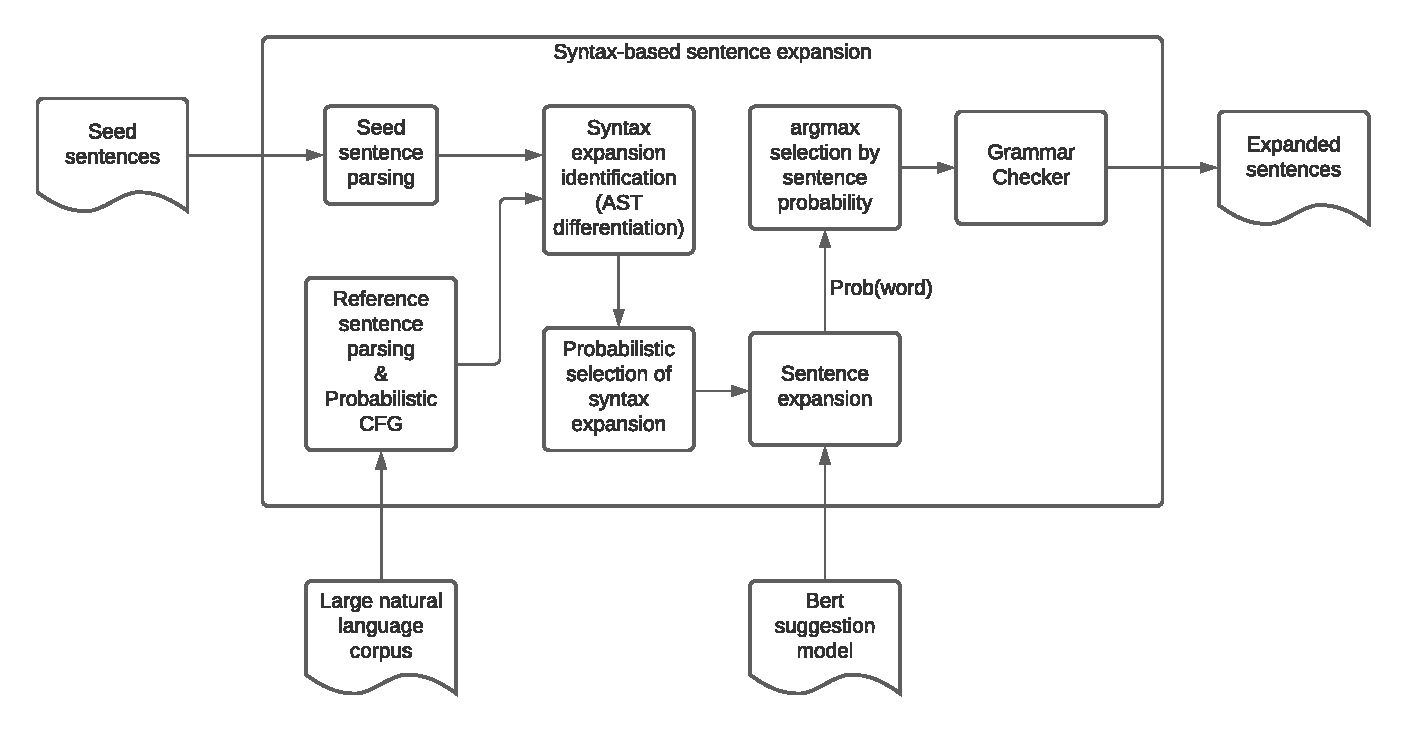
\includegraphics[scale=0.5]{figs/overall.pdf}
  \vspace{-5pt}
  \caption{\OverallModelFigCaption}
  \vspace{-10pt}
\end{figure*}

\Model generates input \sents with the following phases illustrated
in \ref{fig:OverallModel}: 1. search phase searches seed \sents
according to its \req of \lc, 2. seed parsing phase parses the
found seed \sents and extract their \cfg, 3. reference phase
collects large corpus, 4. syntax expansion identification, and
5.\sent expansion and generation. In this section, we provide more
details on each phase.

\subsection{Search phase}
The search phase in \Model searches inputs in dataset and selects
subset of input \sents in the dataset that meets the \lc
\req. The idea behind this phase is that input distribution of
\lc is important to generate inputs relevant to \lc. \Lc explains
expected behaviors of NLP model on specific types of input and
output. The NLP model is evaluated on how much it performs on the
input and output. Thus, \lc introduces the constraints of the input
data. Input data from the constrained distribution are only qualified
to be used for evaluating the NLP model on the \lc.  In addition,
diversity in inputs is important to evaluate NLP models on the
\lc. Inputs that differ are more likely to cover the NLP model
behavior, and more coverage increases trustworthiness of the
evaluation. To generate inputs from same distribution on \lc and high
diversity of inputs, we estabilish \reqs of input and output
for each \lc, and find inputs that fulfil the \reqs. Given a
\lc, a \req consists of search \req, transform
\req and expansion \req. The search \req
describes features and functionalities that we seek to have in
inputs. \Model check each input if it satisfy the \req.

\begin{figure}[t]
  \lstinputlisting[language=json-pretty]{code/requirement_sa1.json}
  \vspace{-10pt}
  \caption{\SearchRequirementExampleFigCaption}
  \vspace{-10pt}
\end{figure}

\begin{figure}[t]
  \lstinputlisting[language=json-pretty]{code/requirement_sa2.json}
  \vspace{-10pt}
  \caption{\TransformRequirementExampleFigCaption}
  \vspace{-10pt}
\end{figure}

Figure~\ref{fig:SearchReqEx} shows \lc of \SareqExOne. To evaluate
this \lc, the input is required to be short and have only \neu \adjs,
\neu \nns. In addition, the label needs to be \neu. Therefore, all
short natural \sents with only \neu \adjs and \neu \nns are available
to evaluate NLP models. Next, transform \req explains how the input
and output needs to be tranfromed. Some \lc only accepts heavily
limited input distribution, and it is unlikely to be included in
searching dataset because of its high structural diversity. Therefore,
our approach is to find inputs by relaxing search requirement and
transform the input to match the target requirement of the \lc. In
this work, the inputs are transformed by word addition or perturbing
the found inputs with \lc dependent templates. \Lc of \SareqExTwo in
the figure~\ref{fig:TransformReqEx}, for instance, requires inputs to
be the negated \pstv \sents and be the neutral expression in the
middle. Finding such \sents is costly because such sentneces are
diverse in terms of their structure. Rather, the \Model search \pstv s
and \neu inputs and combine them into negated \pstv \sents. The
transformation of inputs produce the transformed inputs in
distribution on \lc and high diversity in the inputs because of that
from initially found inputs.
